\documentclass[a4paper,11pt]{article}
%\pagestyle{headings}
\usepackage{svg}

% des paquetages indispensables, qui ajoutent des fonctionnalites
%\usepackage[latin1]{inputenc}
\usepackage[utf8]{inputenc}
%\usepackage[french]{babel}
%\usepackage{lmodern}
\usepackage{amsmath,amssymb}
\usepackage{amsthm}
\usepackage{fullpage}
\usepackage{graphicx}
\usepackage{url}
\usepackage{xspace}
\usepackage{listings}
\usepackage{xcolor}
\usepackage{hyperref}
\usepackage{eurosym}
\usepackage{pdfpages}
\usepackage{tikz}
%\usepackage[yyyymmdd,hhmmss]{datetime}
%\usepackage{dblfloatfix}

%\usepackage{float}
%\floatstyle{boxed}
%\restylefloat{figure}

%configuration de listings pour l'affichage du code
\lstset{
    language=ruby,
    basicstyle=\ttfamily\small, %
    identifierstyle=\color{red}, %
    keywordstyle=\color{blue}, %
    stringstyle=\color{black!60}, %
    commentstyle=\it\color{black!50}, %
    columns=flexible, %
    tabsize=3, %
    extendedchars=true, %
    showspaces=false, %
    showstringspaces=false, %
    %numbers=left, %
    %numberstyle=\tiny, %
    breaklines=true, %
    breakautoindent=true, %
    captionpos=b,
    frame=single
}

% On fera des listes a puce et non a tiret.
%\renewcommand{\FrenchLabelItem}{\textbullet}

\newtheorem{theoreme}{Th\'{e}or\`{e}me}
\newtheorem{definition}{D\'{e}finition}
\newtheorem{exercice}{Exercice}

\newcommand{\tab}{\hspace*{\parindent}}

%Definition de quelques commandes utiles en maths :

% R et N
\newcommand{\R}{\mathbb{R}}
\newcommand{\N}{\mathbb{N}}
\newcommand{\C}{\mathbb{C}}
% derive partielle et congruence
\newcommand{\drond}{\partial}
\newcommand{\congru}{\equiv}
% blocs parenthese, valeur absolue, norme, crochets, accolades
\newcommand{\abs}[1]{\left\lvert#1\right\rvert}
\newcommand{\norm}[1]{\left\lVert#1\right\lVert}
\newcommand{\braces}[1]{\left(#1\right)}
\newcommand{\croch}[1]{\left[#1\right]}
\newcommand{\cbraces}[1]{\left\{#1\right\}}
% blocs parties entieres superieur et inferieur
\newcommand{\entsup}[1]{\left\lceil#1\right\rceil}
\newcommand{\entinf}[1]{\left\lfloor#1\right\rfloor}

\newcommand{\HRule}{\rule{\linewidth}{0.5mm}}

\newcommand{\gitInfo}{
    \IfFileExists{.compil/gitfile.tex}
    {
        \input{.compil/gitfile.tex}
        \begin{tabular}{|ll|}
            \hline
            Commit  & \GITAbrHash \\
            Date    & \GITAuthorDate \\
            Author  & \GITAuthorName \\
            \hline
            Build date    & \today \\
            Build time    & \currenttime \\
            \hline
        \end{tabular}
    }{
        \begin{tabular}{|ll|}
            \hline
            No git info \\
            \hline
            Build date    & \today \\
            Build time    & \currenttime \\
            \hline
        \end{tabular}
    }
}

%\setcounter{secnumdepth}{3}
\setlength{\columnsep}{10mm}


\title{Systèmes distribués : Makefile}
\author{Thibaut Coutelou, Benjamin Michel, Guillaume Perrin, Nicolas Vignes}
\date{\today}

\begin{document}
\maketitle
%\tableofcontents

\setlength{\parskip}{2mm}

\section{Introduction}
Ce rapport a pour but de présenter le travail réalisé dans le cadre du projet
de systèmes distribués, en présentant notamment, le langage et les algorithmes
que nous avons utilisés.

Dans une deuxième partie, nous présenterons les performances de notre
application au travers des différents tests que nous avons réalisés. Cette
partie se constituera principalement de courbes présentant les résultats.

\section{Partie 1 : Présentation du projet}
\subsection{Langage}
Pour réaliser ce projet, nous avons utilisé le langage \textbf{Go}, développé
par Google. Go n'est pas présent nativement sur les machines de l'Ensimag, il
faut donc installer le compilateur ainsi que les bibliothèques sur sa machine.
Cela se réalise facilement en se rendant sur le site
\href{http://golang.org/doc/install#download}{golang.org}.

\subsection{Algorithmes}
Le fonctionnement de notre application de makefile distribués se déroulent en deux parties :
\begin{itemize}
\item Lecture et construction de l'arbre de dépendances à partir du Makefile
    par le client.
\item Exécution des différentes tâches par les workers. Le client envoie les
    différentes tâches aux listeners (en fonction des dépendances) qui lancent
    des workers exécutant celle-ci.
\end{itemize}

\subsection{Structure du code}
Le code source est décomposé en plusieurs fichiers .go visant à créer deux exécutables : listener et client.
\begin{itemize}
\item listener.go : écoute des clients et lancement de workers
\item worker.go : exécution des commandes pour générer les cibles
\item client.go : appel à config et au parser pour les options de config et l'arbre des dépendances puis appels aux workers pour créer les différentes cibles
\item config.go : lecture du fichier de configuration pour préciser les hosts
\item parser.go : construction de l'arbre des dépendances d'un Makefile
\end{itemize}

\section{Partie 2 : Performances}

\begin{figure}[htbp]
  \centering
  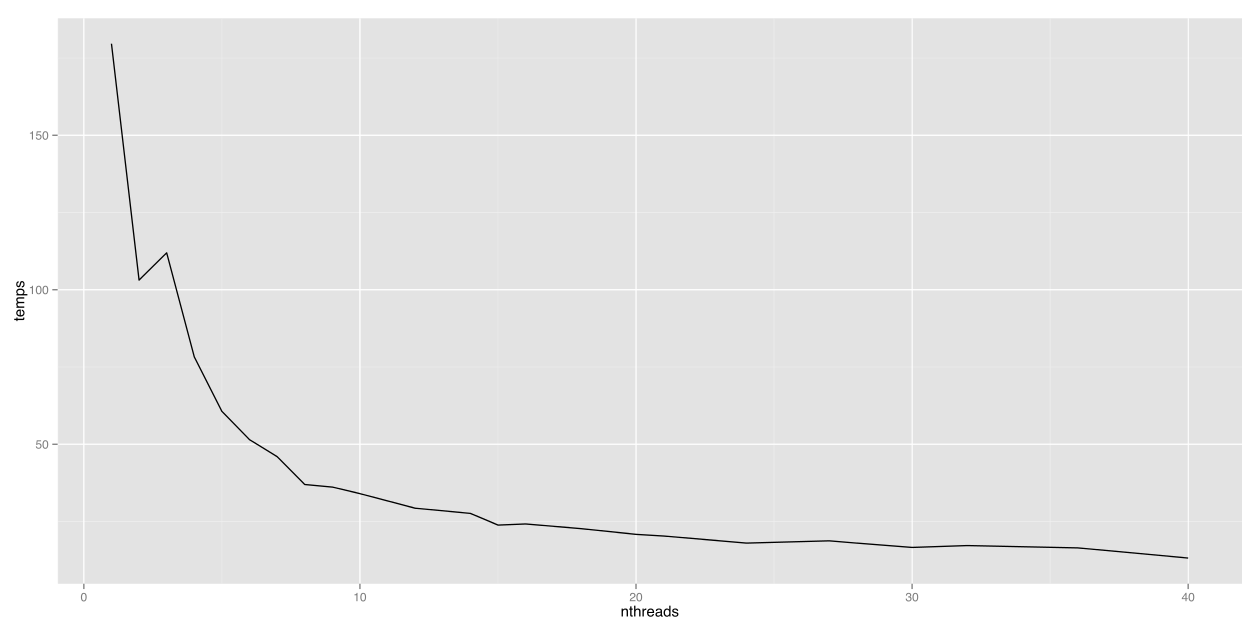
\includegraphics[scale=0.35]{img/blender1_temps.png}
  \caption{Blender 2.49 : Temps}
\end{figure}

\begin{figure}[htbp]
  \centering
  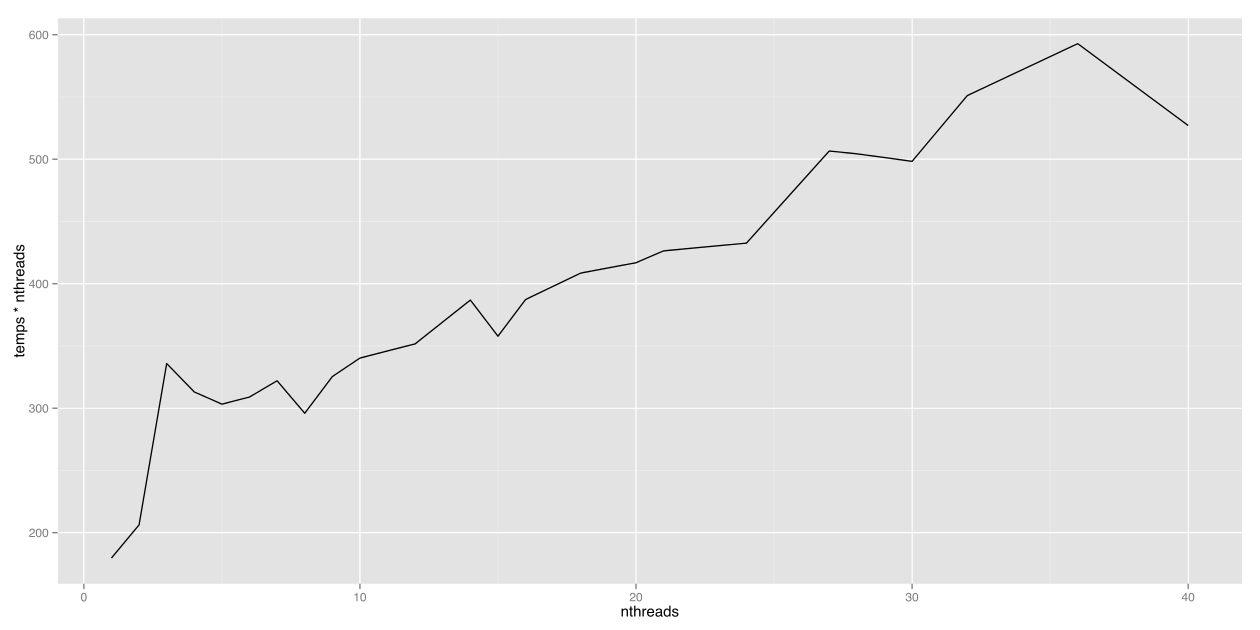
\includegraphics[scale=0.35]{img/blender1_travail.png}
  \caption{Blender 2.49 : Travail}
\end{figure}

\begin{figure}[htbp]
  \centering
  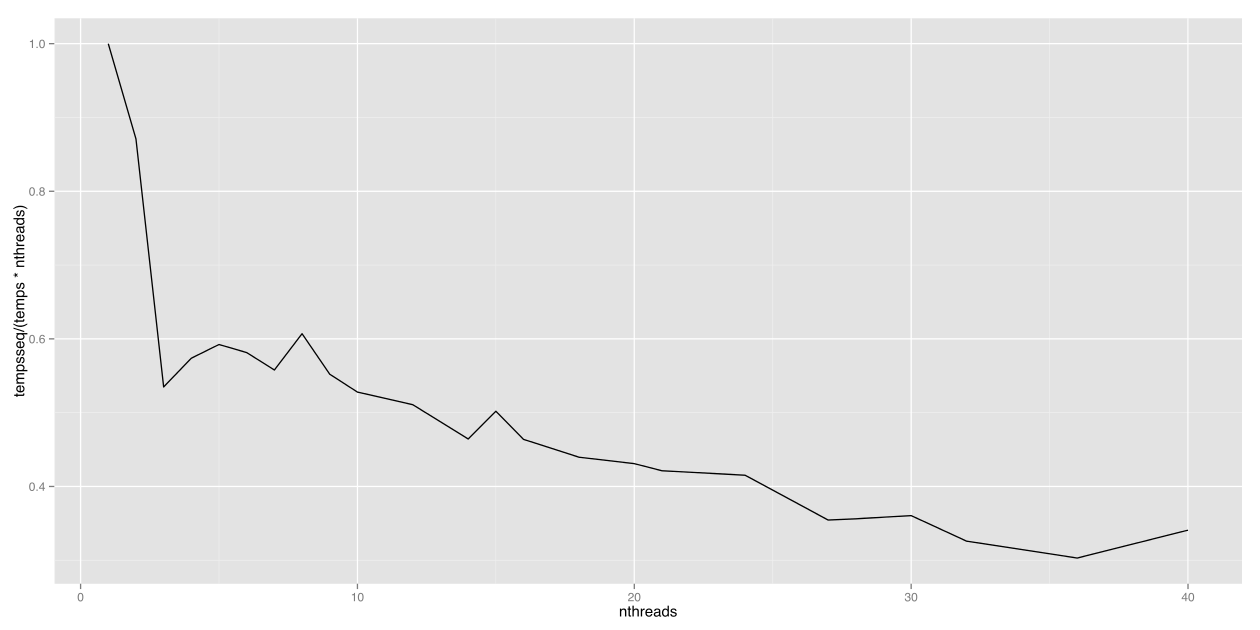
\includegraphics[scale=0.35]{img/blender1_efficacite.png}
  \caption{Blender 2.49 : Efficacite}
\end{figure}

\begin{figure}[htbp]
  \centering
  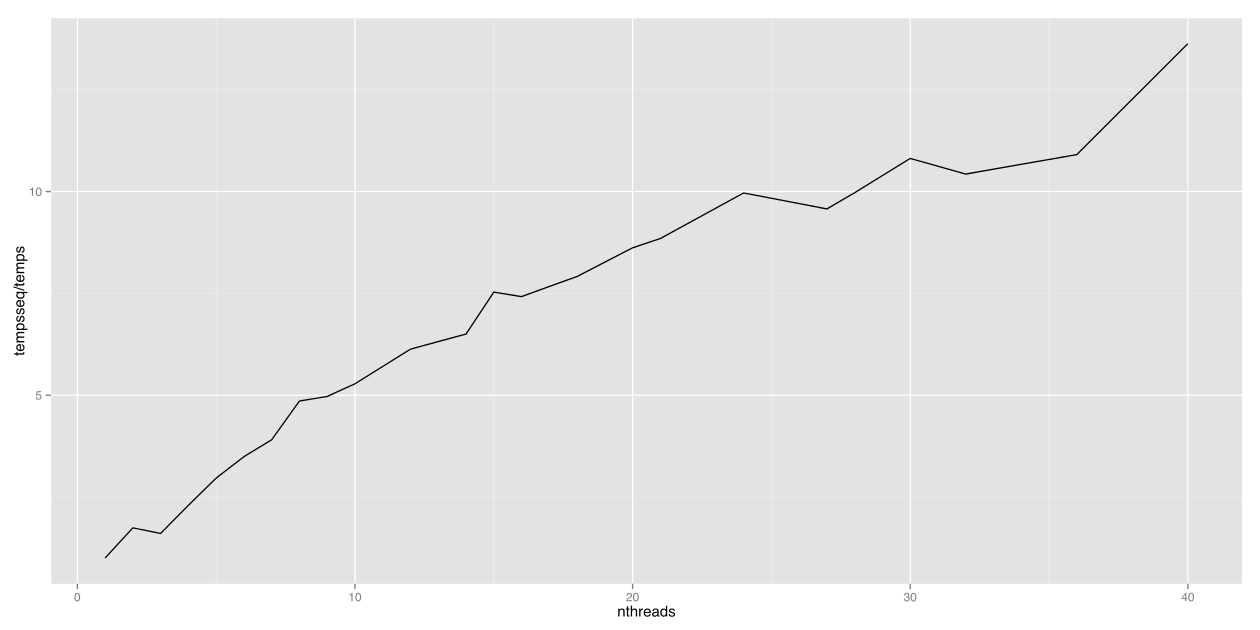
\includegraphics[scale=0.35]{img/blender1_acceleration.png}
  \caption{Blender 2.49 : Accélération}
\end{figure}

\begin{figure}[htbp]
  \centering
  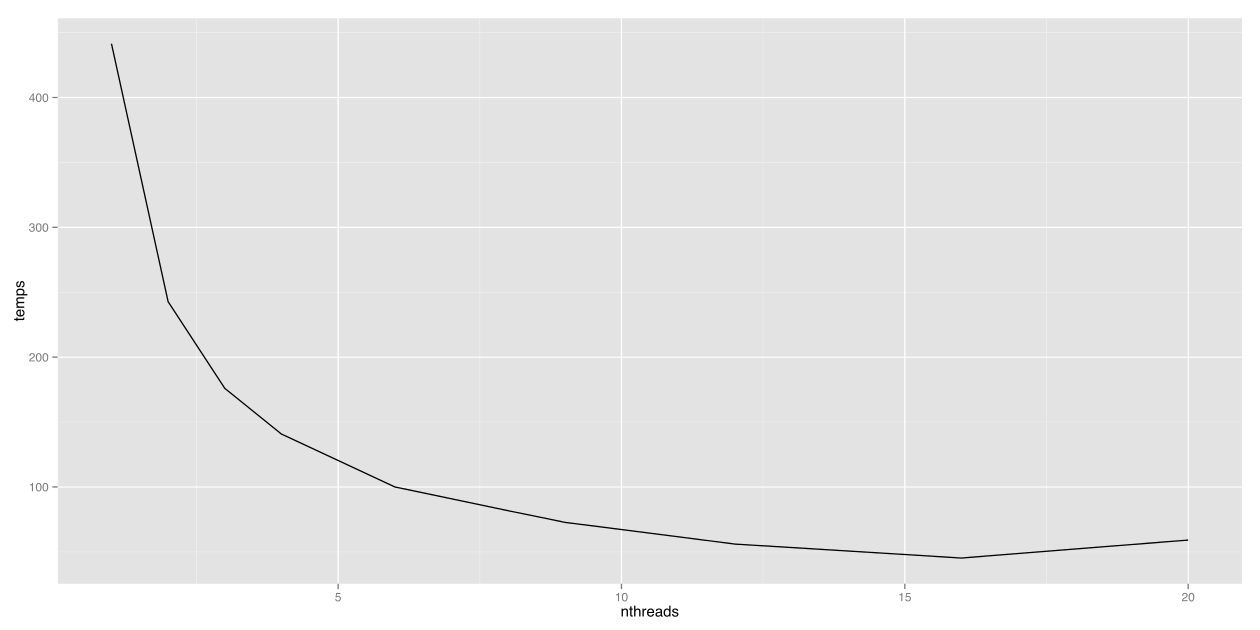
\includegraphics[scale=0.35]{img/blender2_temps.png}
  \caption{Blender 2.59 : Temps}
\end{figure}

\begin{figure}[htbp]
  \centering
  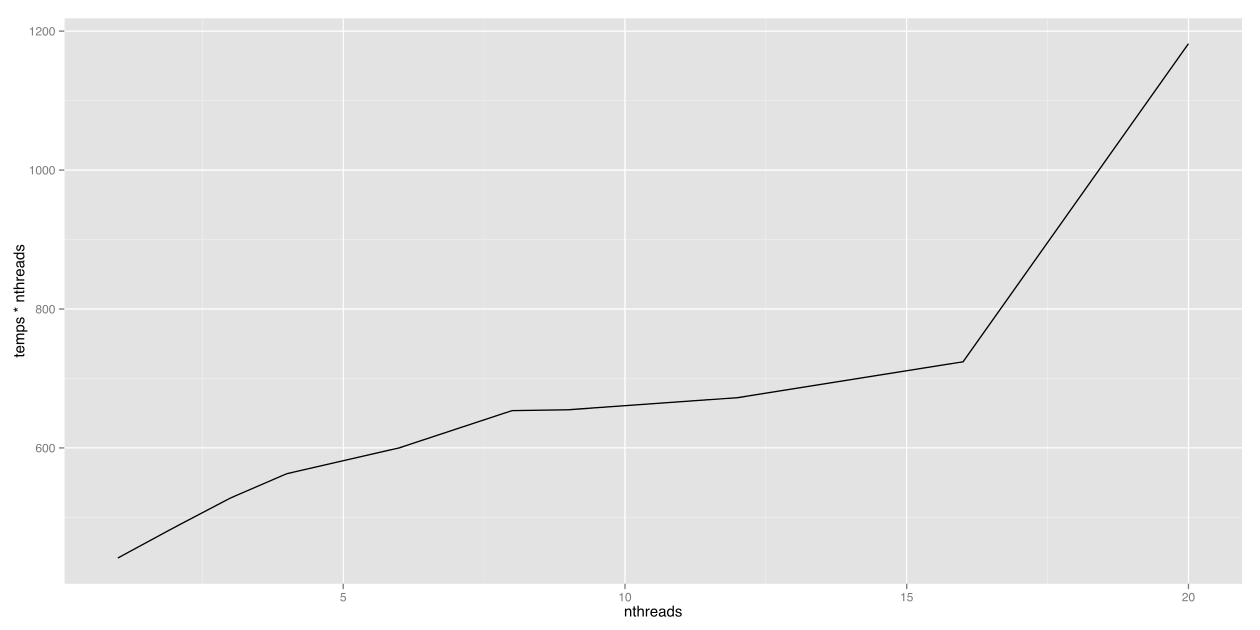
\includegraphics[scale=0.35]{img/blender2_travail.png}
  \caption{Blender 2.59 : Travail}
\end{figure}

\begin{figure}[htbp]
  \centering
  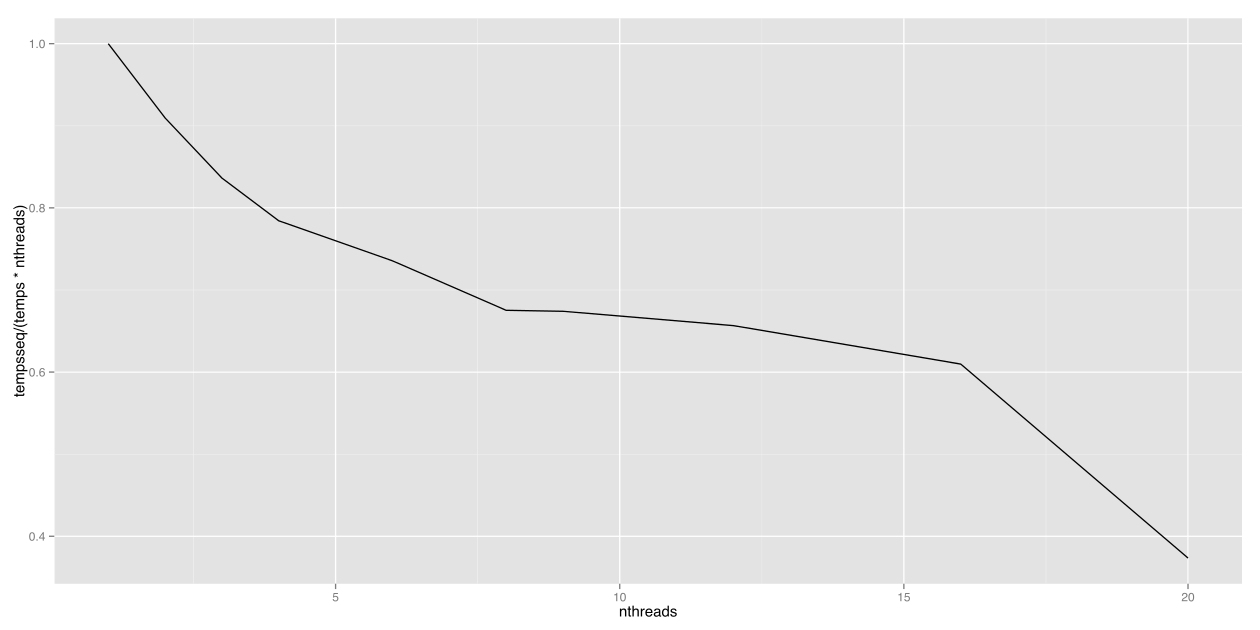
\includegraphics[scale=0.35]{img/blender2_efficacite.png}
  \caption{Blender 2.59 : Efficacite}
\end{figure}

\begin{figure}[htbp]
  \centering
  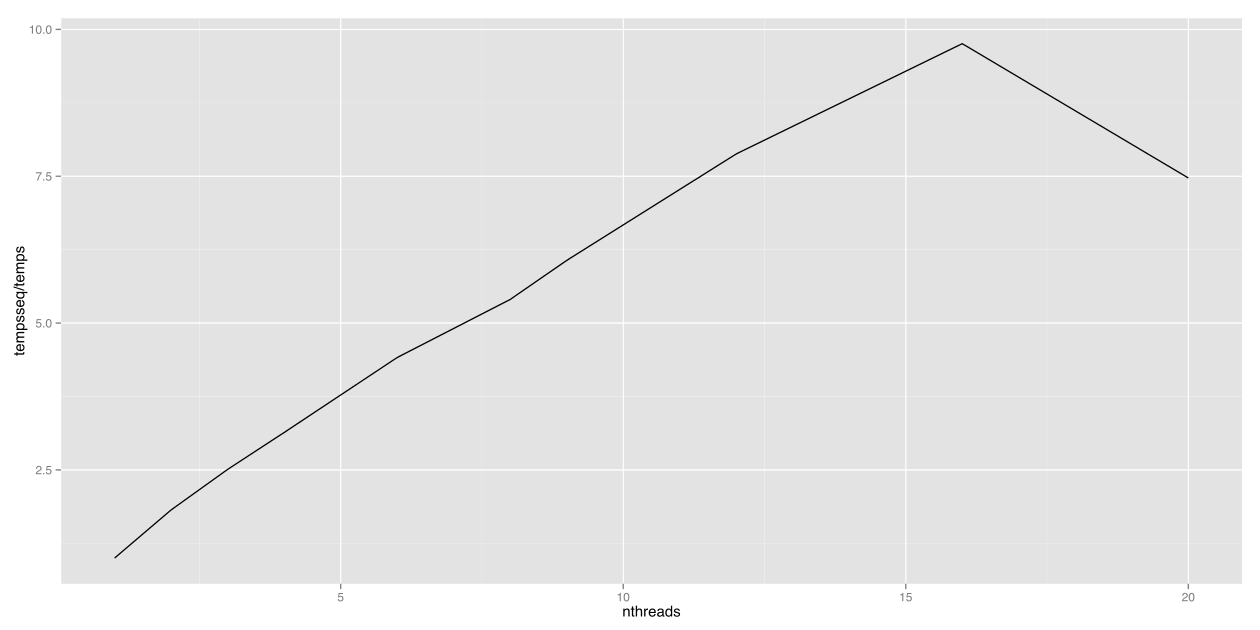
\includegraphics[scale=0.35]{img/blender2_acceleration.png}
  \caption{Blender 2.59 : Accélération}
\end{figure}

\begin{figure}[htbp]
  \centering
  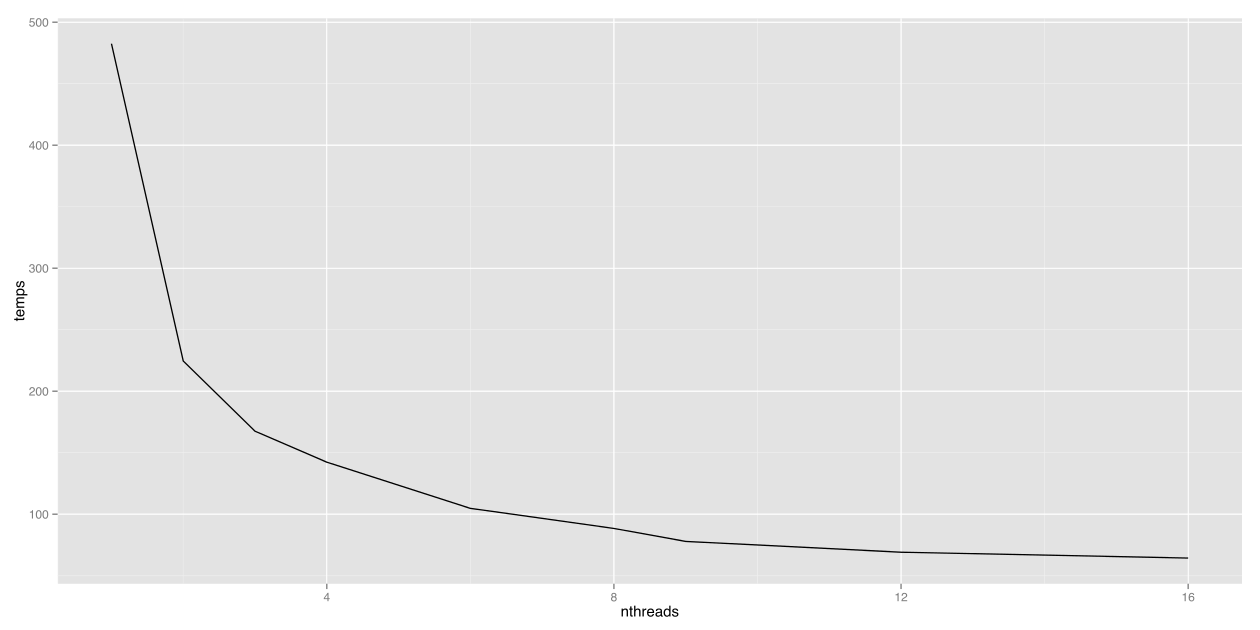
\includegraphics[scale=0.35]{img/premier_temps.png}
  \caption{Premier : Temps}
\end{figure}

\begin{figure}[htbp]
  \centering
  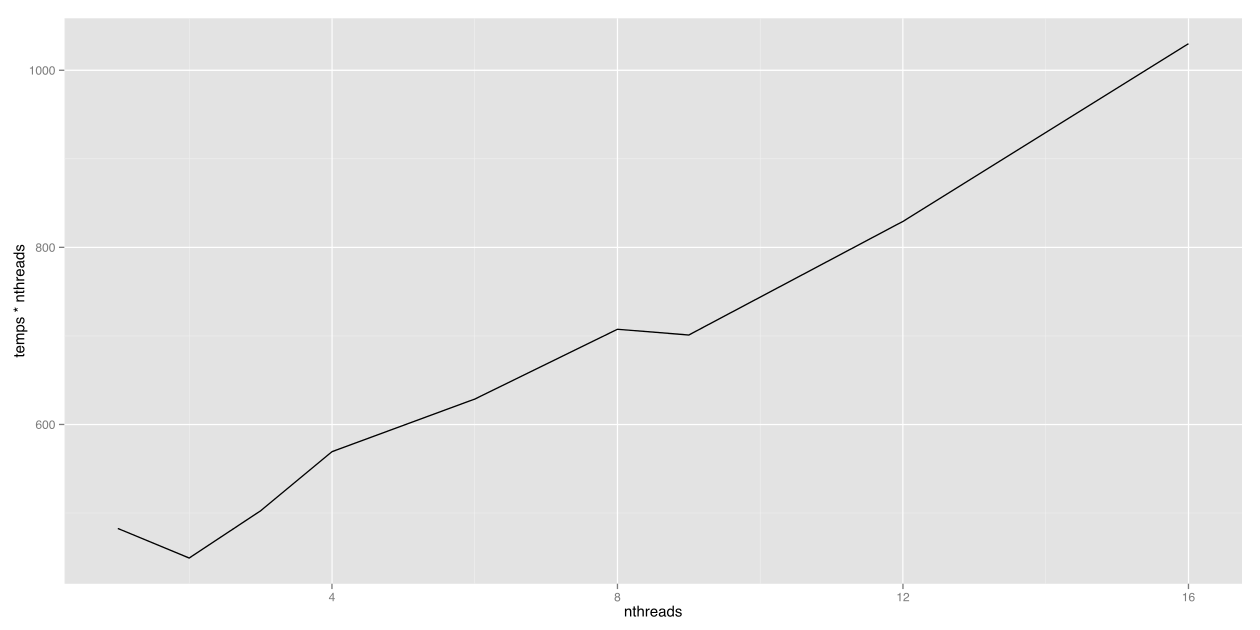
\includegraphics[scale=0.35]{img/premier_travail.png}
  \caption{Premier : Travail}
\end{figure}

\begin{figure}[htbp]
  \centering
  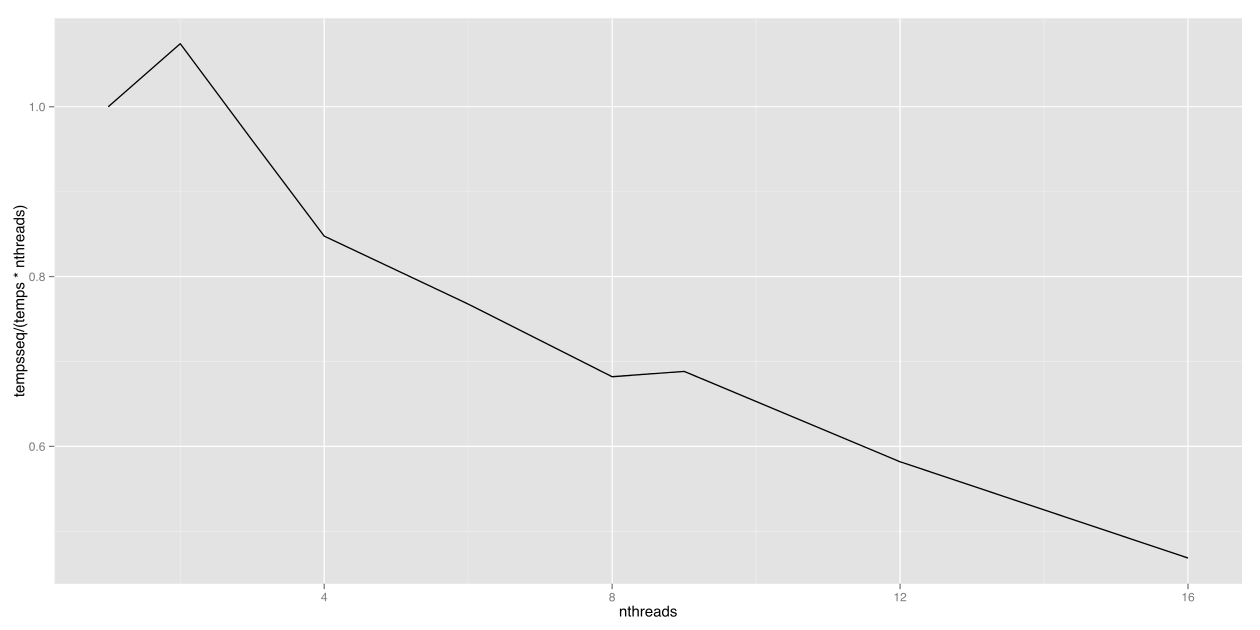
\includegraphics[scale=0.35]{img/premier_efficacite.png}
  \caption{Premier : Efficacite}
\end{figure}

\begin{figure}[htbp]
  \centering
  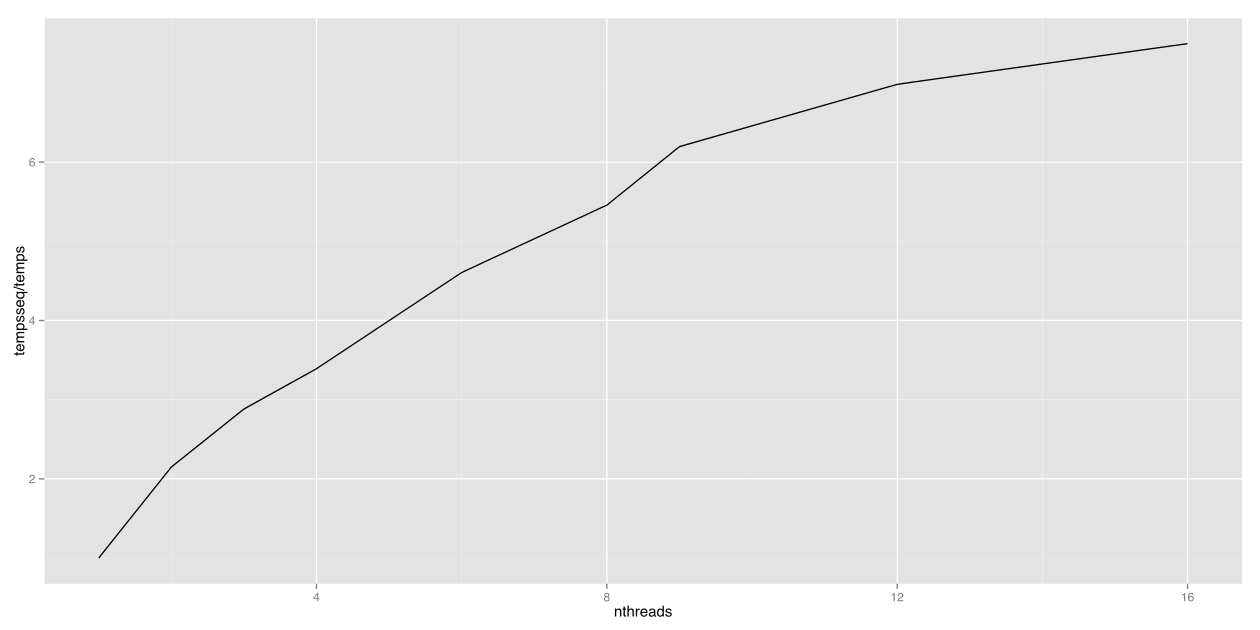
\includegraphics[scale=0.35]{img/premier_acceleration.png}
  \caption{Premier : Accélération}
\end{figure}

\end{document}

% vim: set spell spelllang=fr:
